\documentclass[11pt]{amsbook}

\makeatletter
\def\@thm#1#2#3{%
  \ifhmode\unskip\unskip\par\fi
  \normalfont
  \trivlist
  \let\thmheadnl\relax
  \let\thm@swap\@gobble
  \let\thm@indent\indent % indent
  \thm@headfont{\bfseries}% heading font boldface // changed
  \thm@notefont{\fontseries\mddefault\upshape}%
  \thm@headpunct{.}% add period after heading
  \thm@headsep 5\p@ plus\p@ minus\p@\relax
  \thm@space@setup
  #1% style overrides
  \@topsep \thm@preskip               % used by thm head
  \@topsepadd \thm@postskip           % used by \@endparenv
  \def\@tempa{#2}\ifx\@empty\@tempa
    \def\@tempa{\@oparg{\@begintheorem{#3}{}}[]}%
  \else
    \refstepcounter{#2}%
    \def\@tempa{\@oparg{\@begintheorem{#3}{\csname the#2\endcsname}}[]}%
  \fi
  \@tempa
}
\makeatother

\renewcommand{\chaptername}{Lecture}


\usepackage[T1]{fontenc}
\usepackage[latin1]{inputenc}
\usepackage{times}
\usepackage{microtype}
\usepackage{amssymb}
\usepackage{a4wide}
\usepackage{graphicx}
%\usepackage{paralist}
\usepackage{bbm}
\usepackage{color}
\usepackage[pagebackref]{hyperref} 
\hypersetup{pdftitle={\title}, pdfauthor={\author}}
\usepackage{verbatim}
\usepackage{url}
\usepackage[pagebackref]{hyperref}
\hypersetup{pdftitle={\title}, pdfauthor={\author}}

\usepackage{amsmath}
%\usepackage{mathtools}
\usepackage{tikz}
\usetikzlibrary{matrix,arrows,decorations.pathmorphing}

\newcommand{\ba}{{\boldsymbol{a}}}
\newcommand{\balpha}{{\boldsymbol{\alpha}}}
\newcommand{\bb}{{\boldsymbol{b}}}
%\newcommand{\bc}{{\boldsymbol{c}}}
\newcommand{\be}{{\boldsymbol{e}}}
\newcommand{\bff}{{\boldsymbol{f}}}
\newcommand{\bnu}{{\boldsymbol{\nu}}}
\newcommand{\bm}{{\boldsymbol{m}}}
\newcommand{\bo}{{\boldsymbol{0}}}
\newcommand{\bp}{{\boldsymbol{p}}}
\newcommand{\bq}{{\boldsymbol{q}}}
\newcommand{\br}{{\boldsymbol{r}}}
\newcommand{\bsigma}{{\boldsymbol{\sigma}}}
\newcommand{\bt}{{\boldsymbol{t}}}
\newcommand{\bv}{{\boldsymbol{v}}}
\newcommand{\bw}{{\boldsymbol{w}}}
\newcommand{\bx}{{\boldsymbol{x}}}
\newcommand{\by}{{\boldsymbol{y}}}
\newcommand{\bz}{{\boldsymbol{z}}}
\newcommand{\bone}{{\boldsymbol{1}}}

\newcommand{\RR}{\mathbb{R}}
\newcommand{\Rgeo}{{\mathbb{R}_{\ge0}}}
\newcommand{\Zgeo}{{\mathbb{Z}_{\ge0}}}
\newcommand{\NN}{\mathbb{N}}
\newcommand{\ZZ}{\mathbb{Z}}
\newcommand{\QQ}{\mathbb{Q}}
\newcommand{\CC}{\mathbb{C}}

\newcommand{\cA}{{\mathcal{A}}}
\newcommand{\cC}{{\mathcal{C}}}
\newcommand{\cD}{{\mathcal{D}}}
\newcommand{\cH}{{\mathcal{H}}}
\newcommand{\cL}{{\mathcal{L}}}
\newcommand{\cO}{{\mathcal{O}}}
\newcommand{\cP}{{\mathcal{P}}}

\newcommand{\cU}{\mathcal{U}}
\newcommand{\tU}{\tilde{\mathcal{U}}}
\newcommand{\tV}{\tilde{\mathcal{V}}}

\newcommand{\scp}[2]{\langle #1,#2\rangle}
\newcommand{\fl}[1]{\left\lfloor #1\right\rfloor}
\newcommand{\ce}[1]{\left\lceil #1\right\rceil}
\newcommand{\rcone}[1]{{{}_\Rgeo\!\left\langle #1\right\rangle}}
\newcommand{\zcone}[1]{{{}_\Zgeo\!\left\langle #1\right\rangle}}

\newcommand{\bn}{{\color{blue}\texttt{\bfseries n}}}
\newcommand{\bc}{{\color{blue}$\boldsymbol{\circ}$}}
\newcommand{\rn}{{\color{red}\texttt{\bfseries n}}}
\newcommand{\rs}{{\color{red}\texttt{\bfseries *}}}
\newcommand{\rt}{{\color{red}$\boldsymbol{\times}$}}
\newcommand{\bB}{{\color{blue}\texttt{\bfseries B}}}
\newcommand{\rR}{{\color{red}\texttt{\bfseries R}}}

\newcommand{\crb}[1]{{\color{red}\texttt{\bfseries{#1}}}}
\newcommand{\cbb}[1]{{\color{blue}\texttt{\bfseries{#1}}}}

\DeclareMathOperator{\interior}{int}
\DeclareMathOperator{\relint}{relint}
\DeclareMathOperator{\conv}{conv}
\DeclareMathOperator{\cone}{cone}
\DeclareMathOperator{\aff}{aff}
\DeclareMathOperator{\vol}{vol}
\DeclareMathOperator{\dist}{dist}
\DeclareMathOperator{\vertices}{vert}
\DeclareMathOperator{\rang}{rang}
\DeclareMathOperator{\sign}{sign}
\DeclareMathOperator{\pyr}{pyr}
\DeclareMathOperator{\bipyr}{bipyr}
\DeclareMathOperator{\Sl}{Sl}
\DeclareMathOperator{\im}{Im}
\DeclareMathOperator{\colspan}{colspan}
\DeclareMathOperator{\rank}{rank}

%%%%%%%%%%%%%%%%%%%%%%%%%%%%%%%%%%%%%%%%Ferran%%%%%%%%%%%%%%%%%%%%%%%%%%%%%%%%%%%%%%%%%%%%%%%%%%%%%%%%%%%%%%%%%%%%%%%%%%%%%%%
\newcommand{\Proj}{\mathbb{P}}
\DeclareMathOperator{\id}{id}
\DeclareMathOperator{\Vor}{Vor}
\newcommand{\HH}{\mathbb{H}}

\DeclareMathOperator{\sgn}{sgn} %signum
\DeclareMathOperator{\ggT}{ggT}

\newcommand{\ojo}[1]{\textsf{\bfseries\boldmath #1}}
\newcommand{\scribe}[1]{\begin{center}\emph{Scribe: #1}\end{center}\bigskip}

\graphicspath{{graphics/}}

\numberwithin{equation}{chapter}

\newtheorem{theorem}{\textbf{Theorem}}[chapter]
\newtheorem{lemma}[theorem]{Lemma}
\newtheorem{proposition}[theorem]{Proposition}
\newtheorem{corollary}[theorem]{Corollary}
\newtheorem{conj}[theorem]{Conjecture}
\newtheorem{exercise}[theorem]{Exercise}
\newtheorem{example}[theorem]{Example}
\newtheorem{claim}[theorem]{Claim}

\theoremstyle{definition}
\newtheorem{definition}[theorem]{Definition}
\newtheorem{defn}[theorem]{Definition}
\newtheorem{remark}[theorem]{Remark}
\newtheorem{observation}[theorem]{Observation}
\newtheorem{obs}[theorem]{Observation}

%\includeonly{lecture3}

\begin{document}

\thispagestyle{empty}

\newcommand{\thisyear}{2013}

\
\vfill
\begin{center}
        \Huge \sffamily\bfseries 
        Discrete and Algorithmic Geometry \thisyear
        \medskip
        (Part 2)

\vspace{2cm}
\LARGE
Julian Pfeifle

\vspace{3cm}

\normalfont\LARGE\sffamily
Version of \today

\vspace{5cm}\
\end{center}

This is the preliminary version of the lecture notes for the second
part of \emph{Discrete and Algorithmic Geometry} (Universitat
Polit�cnica de Catalunya), held in the fall semester of \thisyear\ by Ferran
Hurtado and Julian Pfeifle.

\medskip
These notes are fruit of the collaborative effort of all participating
students, who have taken turns in assembling this text. The name of
each scribe figures in each corresponding section.

\medskip
%The main literature for this course consists of
%\cite{Conway-Sloane-3rd}, \cite{Conway-Strauss08}
%and~\cite{Senechal95}. 

\medskip Suggestions for improvements will always be gladly received
by \texttt{julian.pfeifle@upc.edu}.

\vfill\


% Local Variables: 
% mode: latex
% TeX-master: "dag-upc"
% End: 

\tableofcontents

\chapter{Title of the lecture}

\scribe{Your name here}


% Local Variables: 
% mode: latex
% TeX-master: "dag-upc"
% End: 

\chapter{Asymptotic f-vectors of families of polytopes}

\scribe{Cecilia Gir\'on}

In this section we are going to study the \textit{unimodality conjecture} which says that there exists an $l = P(L)\in\mathbb{N}$ such that $f_0\leq f_1 \leq \cdots\leq f_l \leq f_{l+1}\leq \cdots \leq f_{d-1}\leq f_d$. We woould like to know if it is true. 

First, we define the \textbf{$f$-vector} as the vector of the form $(f_0,f_{1},\cdots,f_{d-1})$ where $f_i$ is as defined before in (\ref{eq1}). We will say that it is a \textbf{flag $f$-vector} $(f_s)_s = [d]$ such that $f_s$ count the number of flags $F_{i_1} \subset F_{i_2} \subset \cdots \subset F_{i_k}$ where $s = \{i_1,i_2,\cdots, i_k \}$ and $\dim F_{i_k} = i_k$ \footnote{You can also read about $cd$-index}.

\bigskip
The unimodal conjecture described before is known to be false for simplical polytopes of dimension $d\geq 19$ and for non-simplicial polytopes of dimension $d \geq 8$. The following conjecture is not known to be false. 

\textbf{Restricted unimodal conjecture (Anders Bjorner)}: 
\begin{eqnarray*}
 f_0\leq f_1\leq \cdots \leq f_{\lfloor \frac{d-1}{4}}\rfloor\\
 f_{\lfloor \frac{3(d-1)}{4}\rfloor}\geq \cdots \geq f_{d-1}
\end{eqnarray*} 

Intuitively we are sure that there is no way this conjecture could be false, but there is not proof of this. We don't even know if $f_k\geq \frac{1}{10000}\min\{f_0,f_{d-1}\}$ is true.

\bigskip

\textbf{Exercises done during the lecture 11/11/2013. Each one includes one}


\section{Operations on polytopes}
\begin{itemize}
\item \textbf{Cartesian (direct) product} $P\times Q$.
\item \textbf{Direct sum} $P^d \oplus q^e \subset \mathbb{R}^{d+e}$.
\item $P*Q\subset \mathbb{R}^{d+e+1}$. It is like $\oplus$ but the subspaces are skew (i.e. affine and they have no point on common). For example $\square^1 *\square^1 = Pyr(P)$.
\end{itemize}

\bigskip
\noindent\textsc{Example}: Given $f_k(P)$, calculate the $k$-th entry of $Pyr(P)$:
\begin{eqnarray*}
f(P)&=&(f_0,f_1,\cdots, f_{d-1}\\
f_k(Pyr(P)) &=& (f_0 +1, f_1 + f_0, f_2+f_1, \cdots, f_{d-2}+ f_{d-3}, f_{d-1}+ f_{d-2}, 1+ f_{d-1})
\end{eqnarray*}
\begin{flushright}
$\clubsuit$
\end{flushright}

\bigskip
\begin{itemize}
\item  \textbf{Connected sum} $P^d\#Q^d$ where $P$ has as simplicial face $f$ and $Q$ has a simplicial face $G$. 
\end{itemize}

This last operation is used to join the asymptotic function $f(\square^d)$ and its dual $f(\diamondsuit ^d)$. To make it work, since $\square^d$ has no triangulations in its faces, it is enough to cut away one vertex and, this way, get a simplex. Merging both functions using the connected sum gives place to a new function which is a non-unimodal function.


% Local Variables: 
% mode: latex
% TeX-master: "dag-upc"
% End: 

\chapter{Pick's Theorem; Lattice packings of spheres}

\scribe{Miquel Ra\"{i}ch}

\section{Pick's Theorem}
\begin{theorem}[Pick]
Let $P$ be a lattice polygon in the plane ($P$ is closed, convex, simple and its vertices lie in $\ZZ^{2}$).
The area of $P$ is $$A(P)=\vol_{2}P=I+\frac{1}{2}B-1$$where:\\
$\mbox{    }\mbox{    } I=$ number of interior lattice points of $P$ $=\#\left\{(\mbox{int }P)\cap\ZZ^{2}\right\}$,\\
$\mbox{    }\mbox{    } B=$ number of boundary lattice points of $P$ $=\#\left\{\partial{}P\cap\ZZ^{2}\right\}$
\end{theorem}
\begin{proof}\mbox{[part]}\\
\begin{enumerate}
\item Show that Pick's formula is additive: if $P=P_1\cup{}P_2$, then $$I+\frac{1}{2}B-1=\left(I_1+\frac{1}{2}b_1-1\right)+\left(I_2+\frac{1}{2}B_2-1\right)$$
\begin{align*}A(P)=&A(P_1)+A(P_2)\\
I=I(P)=&I_1+I_2+L-2\\
B=B(P)=&B_1+B_2-2L+2\end{align*}
{\center (Principle of Inclusion-Exlusion $\rightarrow$ M\"obius function)\quad\quad\\[0.3cm]

\begin{minipage}{0.6\textwidth}$\lceil$ This proves:\begin{enumerate}\item Pick$(P_1\cup{}P_2)\Leftarrow$ Pick$(P_1)$, Pick$(P_2)$\\
\item Pick$(P_1)\Leftarrow$ Pick$(P_1\cup{}P_2)$, Pick$(P_2)$ $\rfloor$\end{enumerate}\end{minipage}}\\[0.5cm]

\item Prove it for lattice triangles.\end{enumerate}
\end{proof}

\section{Lattice packings of spheres}

A {\textbf{lattice-packing}} of congruent spheres ($\equiv$ same radius) in $\RR^{d}$ is a packing such that the set $Z=\{\mbox{centers of the spheres}\}$ is a lattice $L$ (free abelian group).

Let $\{v_1, \ldots, v_n\}\in\RR^{d}$ be a generating set for $$M=\left[\begin{array}{ccc}v_1 & \cdots & v_n\end{array}\right]\!\mbox{, then }L=\{M\lambda\colon\lambda\in\ZZ^{n}\}$$
$$M=\overbrace{\left.\left[\begin{array}{cc}1 & \frac{1}{2} \\ 0 & \frac{1}{2}\sqrt{3} \end{array}\!\right]\right\}}^{n}\!d\quad\quad\quad\quad\quad{}M\lambda=\left[\begin{array}{ccc}v_1 & \cdots & v_n\end{array}\right]\!\left[\begin{array}{c}\lambda_1 \\ \vdots \\ \lambda_n \end{array}\right]=\lambda_1{}v_1+\cdots+\lambda_n{}v_n$$\\[0.2cm]

Sphere packing $B_0+L=\{B_0+v\colon{}v\in{}L\}=\{B_0+M\lambda\colon\lambda\in\ZZ^{n}\}$
$$\forall{}p,q\in{}P,\mbox{ }\exists{}D_p, D_q\colon{}D_p\cap{}Dq=\emptyset\quad\quad\quad\quad{}p\in{}P\subset\RR^{d}\mbox{ discrete set of points}$$\\[0.1cm]
Voroni cell of $p$ w.r.t. $P$ is$$\mbox{Vor}(P)=\{y\in\RR^{d}\colon\lVert{}y-p\rVert\leq\lVert{}y-q\rVert\mbox{ }\forall{}q\in{}P\}$$
$\lceil$ Georges Voronoi (s. XIX) $\rfloor$\\[0.3cm]
Voronoi cells are intersections of half spaces$$\mbox{Vor}(P)=\bigcap_{q\in{}P}H_q\quad\quad\mbox{ where }H_q=\{y\in\RR^{d}\colon\lVert{}y-p\rVert\leq\lVert{}y-q\rVert\}$$

\begin{defn}\mbox{ }\\
$\mbox{    }\mbox{    } $polyhedron $\equiv^{def}$ intersection of half-spaces\\
$\mbox{    }\mbox{    } $polytope $\equiv^{def}$ convex hull of a finite point set $\overset{\text{FTPT}}{\equiv}$ bounded polyhedron\\[0.1cm]
{\small \upshape (FTPT: Fundamental theorem of polytope theory)}
\end{defn}\mbox{ }

\begin{enumerate}\item any convex hull of a finite point set is an intersection of half-spaces [easy by calculating convex hull].\\
\item any \underline{bounded} intersection of half-spaces is the convex hull of a finite set of points, unless the intersection is empty.\end{enumerate}\mbox{ }

Any lattice is isomorphic to some $\ZZ^n$, as abelian groups, by the map $v\in{}L\leftrightarrow\lambda\in\ZZ^n\colon{}v=M\lambda$

\mbox{ }\\[1.1cm]
[I will put images another day :P]

% Local Variables: 
% mode: latex
% TeX-master: "dag-upc"
% End: 
 
\chapter{The hexagonal lattice and laminated lattices}
\scribe{Ane Santos}

\section{The hexagonal lattice}

\begin{definition}
  Let $v_1,\ldots,v_n\in \ZZ^{d}$ and the lattice $L= {}_\ZZ\!\left\langle v_1,\ldots,v_n
  \right\rangle=\left\{\sum\lambda_i v_i : \lambda_i \in \ZZ\right\}=
  \left\{M\lambda:\lambda\in \ZZ^{n}\right\}$ with
  $M=\left[v_1,\ldots,v_n\right]\in\ZZ^{d\times n}$. $M$ is called the \emph{generator
    matrix} and ${}_\ZZ\!\left\langle v_1,\ldots,v_n \right\rangle$ the \emph{integer hull} of the
  lattice.
\end{definition}


We will study two variants of the hexagonal lattice:
\[
  A_{2,\RR^{2}}
  \ = \
  \left\{\begin{bmatrix}
        1 & 1/2 \\
        0 & \sqrt{3}/2 \end{bmatrix}\lambda:\lambda\in\ZZ^{2}\right\}, 
    \qquad
  A_{2,\RR^{3}}
  \ = \
  \left\{\begin{bmatrix}
        1 & 0 \\
        -1 & 1 \\
        0 & -1 \end{bmatrix}\lambda:\lambda\in\ZZ^{2}\right\},
\]
with respective generating matrices
$M=\left[\begin{smallmatrix}
      1 & 1/2 \\
      0 & \sqrt{3}/2 \end{smallmatrix}\right]$ and
$M'=\left[\begin{smallmatrix}
      1 & 0 \\
      -1 & 1 \\
      0 & -1 \end{smallmatrix}\right]$. 

Firstly, we study $A_{2,\RR^{3}}$:

\begin{figure}[htbp]
\centering
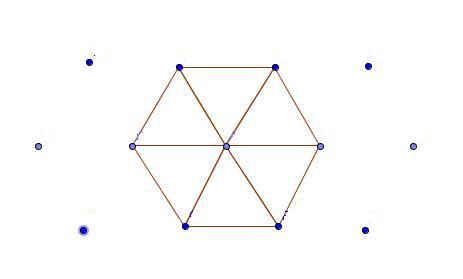
\includegraphics[width=0.5\textwidth]{apunteaklattice}
\caption{$A_{2,\RR^{3}}$}
\end{figure}


\begin{displaymath}
	A_{2,\RR^{3}}=\left\{M'\lambda:\lambda\in\ZZ^{2}\right\}=\left\{\begin{bmatrix}
	\lambda_1 \\
	-\lambda_1 + \lambda_2 \\
	-\lambda_2 \end{bmatrix}:\lambda_1,\lambda_2\in\ZZ\right\}
\end{displaymath}

We want to find a hyperplane that contains $A_{2,\RR^{3}}$. We are in $\RR^{3}$, so this
hyperplane is of the form $\left\{x\in\RR^{3}:\left\langle
    a,x\right\rangle=a_0\right\}$. But we know $0$ is in $A_{2,\RR^{3}}$ so $a_0=0$ and
\[
  H \ = \ 
  \left\{x\in\RR^{3}:\left\langle a,x\right\rangle=0\right\} 
  \ = \ 
  \left\{\omega\in\RR^{3}:\left\langle \omega,x\right\rangle, \forall \in \colspan
    M\right\},
\]
 where $\colspan
M={}_\RR\!\left\langle v_1,\ldots,v_n \right\rangle=\im M$ (it is an abelian group and it is
also a vector space). So, $H=\left\{x\in\RR^{3}: \left\langle
    a,x\right\rangle=0\right\}=\ker M$

$\dim \im M=2$ and $\dim A_{2,\RR^{3}}=3$ $\Longrightarrow$ $\dim A_{2,\RR^{3}}=\dim \ker M +\dim \im M$ $\Longrightarrow$ $\dim \ker M=1$

A generator of $\ker M$ will be $\left(\begin{smallmatrix}
1 \\
1 \\
1 \end{smallmatrix}\right)$

$\left[1 1 1\right]\left[\begin{smallmatrix}
1 & 0 \\
-1 & 1 \\
0 & -1 \end{smallmatrix}\right]=\left[0 0\right]$ $\Rightarrow$ $\ker M= {}_\RR\!\left\langle \left[1 1 1\right]\right\rangle$

So $A_{2,\RR^{3}}\subset\left\{x\in\RR^{3}: x_1+x_2+x_3=0\right\}=\left\{x\in\RR^{3}: \mathbbm{1}x=0\right\}$


\begin{definition}
The \emph{Gram matrix} of a lattice $L$ with generator matrix $M$ is $G_L=M^{T}M$.
\end{definition}


\begin{definition}
The \emph{determinant of a lattice} $L$ with generator matrix $M$ is the determinant of the Gram matrix.
$\det L=\det M^{T}\cdot \det M=\left(\det M\right)^{2} $
\end{definition}


\begin{observation}
 $G_L$ is always a symmetric matrix because $G_L^{T}=\left(M^{T}M\right)^{T}=M^{T}M$.
\end{observation}


We calculate the determinants of $A_{2,\RR^{2}}$ and $A_{2,\RR^{3}}$:

\begin{eqnarray*}
  \det A_{2,\RR^{2}}
  &=&
  \det \begin{bmatrix}
      1 & 0 \\
      \tfrac12 & \tfrac12\sqrt{3} \end{bmatrix}\cdot\begin{bmatrix}
      1 & \tfrac12 \\
      0 & \tfrac12\sqrt{3} \end{bmatrix}
    \ = \ 
    (\tfrac12\sqrt{3})(\tfrac12\sqrt{3})
  \ = \ 
  \frac34,
  \\
  \det A_{2,\RR^{3}}
  &=&
  \det \begin{bmatrix}
      0 & -1 & 0 \\
      0 & 1 & -1\end{bmatrix}\cdot\begin{bmatrix}
      1 & 0 \\
      -1 & 1 \\
      0 & -1 \end{bmatrix}=\det \begin{bmatrix}
      2 & -1 \\
      -1 & 2 \end{bmatrix}
  \ = \
  3.
\end{eqnarray*}

\begin{definition}
The \emph{minimum norm} of a lattice $L$ is $\mu_L=\min\left\{\left\|v\right\|^{2}:v\in L\backslash \left\{0\right\}\right\}$
\end{definition}

From the minimum norms $\mu_{A_{2,\RR^{2}}} = 1$, $\mu_{A_{2,\RR^{3}}} = \sqrt{2}$, we
conclude that both the determinants and the minimum norms of $A_{2,\RR^{2}}$ and
$A_{2,\RR^{3}}$ are different. However, we should not conclude that these lattices are
really different:


\begin{definition}
Two lattices are \emph{isomorphic} if one is obtained from the other by rotation, reflection, translation and scaling.
\end{definition}

The most general map between isomorphic lattices is therefore of the form
\[
   x\ \longmapsto \ \alpha A+t, \qquad\text{where }
   t\in\RR^{n},\; A\in O(n),\; \alpha\in\RR^{*}.
\]
Note that negative $\alpha$ correspond to reflections.

\begin{definition}[Packing density of L]
  $\Delta_L=\frac{\vol(\text{sphere in packing})}{\vol(\Pi_L)=\sqrt{detL}}$,
  where $\Pi_L=\left\{\sum\lambda_i v_i : \lambda_i\in\left[0,1\right)\right\}$ is the
  fundamental parallelopiped.
\end{definition}

To calculate the packing density of $A_{2,\RR^{2}}$ and $A_{2,\RR^{3}}$, note that in
$A_{2,\RR^{2}}$ the radius of the sphere is~$\frac{1}{2}$ so the volume is
$\left(\frac{1}{2}\right)^{2}\pi$. We obtain the same density, which is as it should be
for isomorphic lattices:
\begin{eqnarray*}
  \Delta_{A_{2,\RR^{2}}}
 &=&
  \frac{\left(\frac{1}{2}\right)^{2}\pi}{\sqrt{3/4}}
  \ = \
  \frac{\pi}{2\sqrt{3}},
 \\
  \Delta_{A_{2,\RR^{3}}}
 &=&
  \frac{\left(\frac{1}{2}\sqrt{2}\right)^{2}\pi}{\sqrt{3}}
  \ = \
  \frac{\pi}{2\sqrt{3}}.
\end{eqnarray*}

The connection between these two representations is via the map
\[
 \begin{bmatrix}
1 & \frac{-1}{\sqrt{3}} \\
-1 & \sqrt{3} \\
0 & \frac{-2}{\sqrt{3}}\end{bmatrix}
\begin{bmatrix}
1 & \frac{1}{2} \\
0 & \frac{\sqrt{3}}{2}
\end{bmatrix}
\ = \
\begin{bmatrix}
1 & 0 \\
-1 & 1 \\
0 & 1\end{bmatrix}.
\]

So, we have two different ways to write the same lattice. The advantages of $M'$ over $M$
are that the coordinates are nicer and the symmetries of the lattice are more easily seen.


\begin{claim}
Any permutation of the coordinate axes in $\RR^{3}$ is a symmetry of $A_{2,\RR^{3}}$.
\end{claim}


\begin{proof}
  Let $P:\RR^{2}\longrightarrow\RR^{3}$ be a symmetry of $L=A_{2,\RR^{3}}$, so that
  $P(L)=L$. This means that for all $x\in L$, we should have $P(x)\in L$, which is in turn
  equivalent to the condition that for all $\lambda\in\ZZ^{2}$, there must exist
  $\beta\in\ZZ^{2}$ such that
  \begin{equation}\label{eq:beta}
    M\beta
    \ = \
    PM\lambda.
  \end{equation}
  (In particular, this coordinatizes $x\in L$ as $x=M\lambda$).

  We want to prove that if $P$ is a permutation, then for any $\lambda\in\ZZ^{2}$ we can
  always find a~$\beta\in\ZZ^2$ that makes equation~\eqref{eq:beta} true.  We know $P$,
  $M$ and $\lambda$, so we have to find $\beta$. This is a linear equation for~$\beta$.
  We must show that the linear equation $M\beta=b$ has a unique solution for any
  $b=b_\lambda =PM\lambda$.  The solution is unique if $\rank M$ is maximal, i.e. $\rank
  M=2$. By inspection, $M$~really has rank 2, so we only have to see if it always has a
  solution.  From the Fundamental Theorem of Linear Algebra (part 2)
  \cite{strang-linear-algebra},~\cite{strang-ftla}, the
  system~\eqref{eq:beta} has a solution if and only if
\begin{eqnarray*}
  && b\in \colspan M=\im M 
  \\ &\Longleftrightarrow&
  b\bot\left(\colspan M\right)^{\bot}
  \\ &\Longleftrightarrow&
  b^{T}y=0 \text{ whenever } y\bot \colspan M 
  \\ &\Longleftrightarrow&
  b^{T}y=0 \text{ whenever } y^{T}M=0.
\end{eqnarray*}
Since  $\left[y_1 y_2 y_3\right]\left[\begin{smallmatrix}
1 & 0 \\
-1 & 1 \\
0 & -1\end{smallmatrix}\right]=\left[y_1 - y_2, y_2 - y_3\right]$, we conclude that
$y^{T}M=0$ if and only if
\[
0 y=\alpha\mathbbm{1}
b^{T}y=\lambda^{T}M^{T}P^{T}\alpha\mathbbm{1}=\alpha\lambda^{T}M^{T}P^{T}\mathbbm{1}=\alpha\lambda^{T}M^{T}\mathbbm{1};
\]
but $M^{T}\mathbbm{1}=0$ because $\mathbbm{1}$ is in the $\ker$ of $M$.
\end{proof}


\section{Laminated lattices}


Define $\mathbb{L}_0=\left\{L^{0}\right\}$, $L^{0}=\left\{0\right\}=\mathbb{R}^{0}$ the
zero dimensional lattice and $m:=4$ (usually $m$ is 4 because then the spheres in the
corresponding lattice packing have radius 1).

For $n>0$, $\mathbb{L}_{n+1}=\left\{L_1^{n+1},\ldots,L_{a_n}^{n+1}\right\}$ is the collection of $n+1$-dimensional lattices such that
\begin{enumerate}
\item each $L_i^{n+1}$ has constant minimal norm $m$
\item each $L_i^{n+1}$ contains at least one $L_j^n$ as a sublattice
\item each $L_i^{n+1}$ has minimal determinant subject to (1), (2)
\end{enumerate}


We will see which are these lattices:

\begin{description}
\item[$\mathbb{L}_1$] This lattice must be of the form  $k\ZZ$.
It needs minimal norm $m=4$, so we must take $2\ZZ$, which satisfies (2) and (3).
So the unique laminated lattice of rank~1 is $2\ZZ$.


\item[$\mathbb{L}_2$] Taking $M=\left[\begin{smallmatrix}
      2 & 0 \\
      0 & 2\end{smallmatrix}\right]$ satisfies (1),(2) and (3), and yields
  $2\ZZ^{2}$. However, it is not necessary that our laminated lattice contain only integer
  points, the only condition is that it must contain~$2\ZZ$. Thus, we have the two
  candidates $2\ZZ^{2}$ and $A^{2}$. We decide between the two by
  calculating the determinant corresponding to the generator matrices $M_1=
  \left[\begin{smallmatrix}
    4 & 0\\
    0 & 4
  \end{smallmatrix}\right]$ and $M_2 = \left[\begin{smallmatrix}
        2 & 1 \\
        0 & \sqrt{3} \end{smallmatrix}\right]$:
  \begin{eqnarray*}
    \det 2\ZZ^{2} 
    & = & 
    \det M_1^{T}M_1 \ = \ \det\begin{bmatrix}
        4 & 0 \\
        0 & 4 \end{bmatrix} \ = \ 16;
      \\
    \det A_2
    &=& 
    \det M_2^{T}M_2 \ = \ \det\begin{bmatrix}
        4 & 2 \\
        2 & 4 \end{bmatrix} \ = \ 12.
\end{eqnarray*}
We see that $\det A_2 < \det 2\ZZ^{2}$, which comes about because the area of the
fundamental parallelopiped for $A_2$ is less than that of the square. So $\mathbb{L}_2$
is~$A_2$.
\end{description}
We will see now how can we do the sphere packing:

\begin{figure}[htbp]
\centering
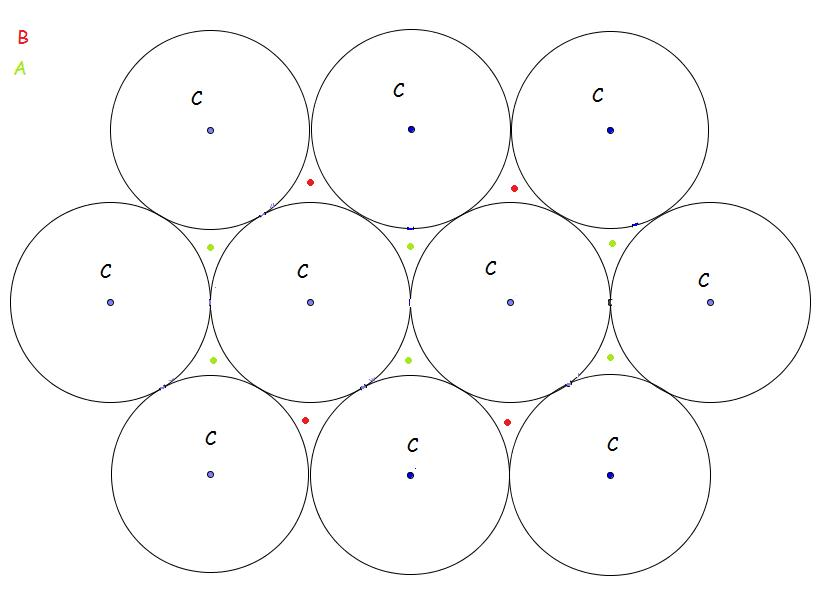
\includegraphics[width=0.5\textwidth]{apunteslattice}
\caption{sphere packing}
\end{figure}

For the next layer we have two options, put them (the centers of the sphere) over the deep holes A or over the deep holes B. For the second layer we put, we will have the possibility of putting them over C (the centers of the spheres of the first layer).
Each lattice obtained by snugly packing copies of $A_2$ is determied by the sequences
ABAB.... (this is the hexagonal close packing(He attoms))
ABCABC....(this is the face-centered cubic lattice ($A_3$))
of equivalence classes of deep holes.

In each step there are two options to choose from, which makes uncountably many possibilities in total.



% Local Variables: 
% mode: latex
% TeX-master: "dag-upc"
% End: 

\setcounter{chapter}{5}
\chapter{Some basic concepts in geometry and software; Introduction to Packings}

\scribe{Ferran Dachs Cadefau}


For the first part see \cite{Pfeifle}.
\section{Big numbers}

Using computers, you can represent big numbers, you can do: 

\renewcommand{\arraystretch}{1.5}
\begin{tabular}{|c|c|c|}
\hline
$\NN$, $\ZZ$	 	&\texttt{int, long int, long long int} 			&$-9.2 \cdot 10^{18} ... 9.2 \cdot 10^{18}$	\\
			&or work with arbitrary precision (slower)		&\texttt{gmplib.org}				\\
\hline
$\QQ$			&$\{(n, d) : n \in \ZZ, d \in \NN_{>0} \}/\sim$		&\texttt{gmplib.org}				\\
			&where $(n, d) \sim (n' , d' )$ iff $nd' = n'd$		&						\\
\hline
$\RR$			&algebraic numbers ok ( $\sqrt{2}$, $\sqrt[4]{3}$),	&\texttt{cgal.org, mpfr.org}			\\
			&transcendental ones not ($\pi$, e)			&						\\
\hline
$\CC$, $\HH$		&pairs or quadruples of reals				&\texttt{\#include <complex>}			\\
\hline
\end{tabular}


But how to represent very big numbers? For example using 4 symbols what is the biggest number that you can represent?

$$10^{99} < 9^{999} < 9^{9^{9^9}} = 9 \uparrow 4 < 9 \uparrow 9 \uparrow 9 \uparrow 9 = 9 \uparrow \uparrow 4 < 9 \Uparrow 9 \Uparrow 9 \Uparrow 9$$

This is known as Knuth's up-arrow notation, to represent bigger numbers there are the Ackerman Function:

$$A(k,n) = n \Uparrow^{(k)} n$$
$$A(n,n) = n \Uparrow^{(n)} n$$

For example:

$$A(2)= 2 \Uparrow 2 = 2 \uparrow 2 \uparrow 2 = 2 \uparrow \left( 2^2\right) = 2^{2^{2^2}}$$
$$A(3)= 3 \Uparrow^{(3)} 3 = 3 \Uparrow 3 \Uparrow 3 \Uparrow 3$$

Using this we can define $\alpha(x)$ as:

$$\alpha(x)=\max\{n\in\NN_{\geqslant 1}:A(n)<x\}$$

It appears, for example, in the complexity of the lower envelope of a segment arrangement. In the plane is $\Omega(n\alpha(n))$

\section{Projective geometry and Polarity}
\subsection{Projective geometry}

We define the projective space as:

$$\begin{array}{rcl}
   \Proj^n	&=	&\{\text{lines through }0\in\RR^{n+1} \}	\\
		&=	&S^n/\ZZ_2
  \end{array}
$$

We are identifying the antipodes: $x$ and $-x$. But we have a problem: $\Proj^1$, $\Proj^3$ are orientable, but for example $\Proj^2$ not: we can't define interior (inside/outside), therefore we can't define convex.

In $\Proj^2$ The line through points $p_1$ and $p_2$:

\begin{itemize}
\item $p_1$ lies on $l$: $p_1\perp l$
\item $p_2$ lies on $l$: $p_2\perp l$
\end{itemize}

Therefore: $l = \lambda \cdot  p_1 \times p_2$ ($\times$ is the cross-product of vectors in $\RR^3$, in higher dimensions is the determinant).

The point $q$ on lines $l_1$ and $l_2$:

\begin{itemize}
\item $q$ lies on $l_1$: $q\perp l_1$
\item$q$ lies on $l_2$: $q\perp l_2$
\end{itemize}

Therefore: $q = \lambda \cdot l_1 \times l_2$ (the cross-product of vectors in $\RR^3$, in higher dimensions is the determinant).

Computationally, we can intersect lines and join points, in homogeneous coordinates or in Cartesian coordinates. In the first case we have:

\texttt{void intersect\_lines(const vec\_t\& l1, const vec\_t\& l2, vec\_t\& p)}

\texttt{\{}

\quad\texttt{cross\_product(l1, l2, p);}

\texttt{\}}

\texttt{void join\_points(const vec\_t\& p1, const vec\_t\& p2, vec\_t\& l)}

\texttt{\{}

\quad\texttt{cross\_product(p1, p2, l);}

\texttt{\}}

\texttt{void cross\_product(const vec\_t\& l1, const vec\_t\& l2, vec\_t\& p)}

\texttt{\{}

\quad\texttt{p[0] = l1[1]*l2[2] - l1[2]*l2[1];}

\quad\texttt{p[1] = -l1[0]*l2[2] + l1[2]*l2[0];}

\quad\texttt{p[2] = l1[0]*l2[1] - l1[1]*l2[0];}

\texttt{\}}

This code is \textbf{correct} (calculates exactly what it should), \textbf{efficient} (No extraneous copying (\&) and reuse of code), and \textbf{robust} (No influence of rounding errors and it handles all cases, even degenerate ones).


But, in Cartesian coordinates. A line is now $y = kx + d$, stored as a vector $(k , d)$.

\texttt{bool intersect\_lines(const vec\_t\& l1, const vec\_t\& l2, vec\_t\& p)}

\texttt{ \{}

\texttt{if (l1[0]==l2[0]) \{}

\texttt{if (l1[1]==l2[1]) \{}

\texttt{return COINCIDENT\_LINES;}

\texttt{\}}

\texttt{return PARALLEL\_LINES;}

\texttt{\}}

\texttt{p[0] = (l2[1]-l1[1])/(l1[0]-l2[0]);}

\texttt{p[1] = l1[0]*p[0] + l1[1];}

\texttt{\}}

This code is \textit{somewhat} \textbf{efficient} (Again, no copying, but: no reuse of code for join\_points), \textbf{not robust} (It's unstable numerically (==, /)), and \textit{not even} \textbf{correct} (It doesn't handle parallel lines, but that's Euclidean geometry's fault).


\subsection{Polarity}

It's related to \underline{Projective duality}, points are dual to hyperplanes:

$$\begin{array}{rcl}
    \Proj^n(\RR)	&\stackrel{d}{\longrightarrow}	&\left(\Proj^n(\RR)\right)^{\star}\\
    p			&\longmapsto				&p^{\star}
  \end{array}$$

A duality is an involutory order-anti-isomorphism (Involution: $d^2=\id$, isomorphism: bijection collineation, order-anti: $p\in l$ implies $p\supset l$).

The polarity is the same except by convexs.

Polarity send: points to half-spaces. Given $a\in \RR^n$:
$$a\mapsto H_a=\{x\in\RR^d:\langle a,x\rangle\leqslant 1\}\leftrightarrow x\supset (\RR^d)^{\star}$$

Equivalently, they identify points with hyperplanes via homogeneous coordinates.

For example, if we take $p=(a:b:1)\in \overrightarrow{\Proj^2}$ a point, then $p^{\star}=(a:b:1)\in \left(\overrightarrow{\Proj^2}\right)^{\star}$ a line, and $p^{\star\star}=p$.

$P\in l\Leftrightarrow p\perp l\Leftrightarrow p^{\star}\perp l^{\star}\Leftrightarrow l^{\star}\perp p^{\star}\Leftrightarrow l^{\star}\in p^{\star}$ 

\section{Polymake}

Polymake is a free program in perl. For example we can define a cube in dimension 3 as:

\texttt{polytope > \$p=cube(3);}

Another thing is to know properties about a polytope. For example the coordinates of the vertices:

\texttt{polytope > print \$p->VERTICES;}

\texttt{1 -1 -1 -1}

\texttt{1 1 -1 -1}

\texttt{1 -1 1 -1}

\texttt{1 1 1 -1}

\texttt{1 -1 -1 1}

\texttt{1 1 -1 1}

\texttt{1 -1 1 1}

\texttt{1 1 1 1}

Or the number of faces of each dimension:

\texttt{polytope > print \$p->F\_VECTOR;}

\texttt{8 12 6}

Or the vertices in each facet:

\texttt{polytope > print \$p->VERTICES\_IN\_FACETS;}

\texttt{\{0 2 4 6\}}

\texttt{\{1 3 5 7\}}

\texttt{\{0 1 4 5\}}

\texttt{\{2 3 6 7\}}

\texttt{\{0 1 2 3\}}

\texttt{\{4 5 6 7\}}

To see a representation of the polytope you can execute:

\texttt{polytope > \$p-> VISUAL;}

\begin{figure}[htbp]
  \centering
  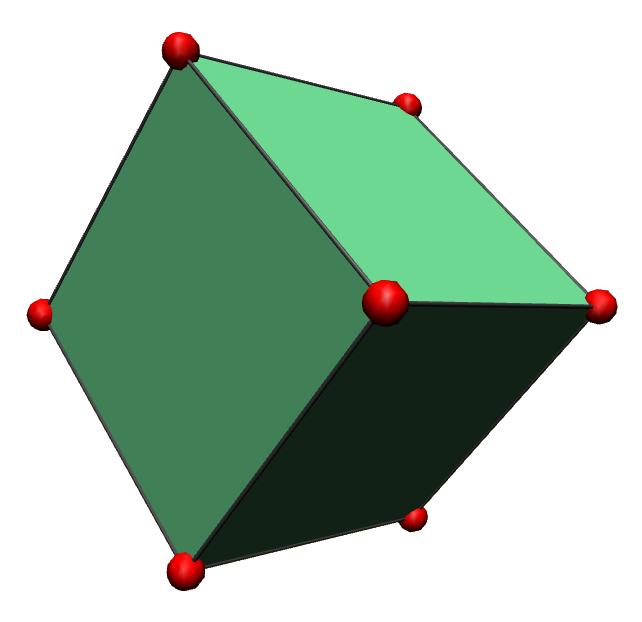
\includegraphics[width=.5\linewidth]{l6_cube.png}
  
  \caption{The representation of the cube in dimension 3 due with Polymake}
\label{fig:l6:1}
\end{figure}

To see a representation of graph of the polytope you can execute:

\texttt{polytope > \$p-> VISUAL\_FACE\_LATTICE;}

\begin{figure}[htbp]
  \centering
  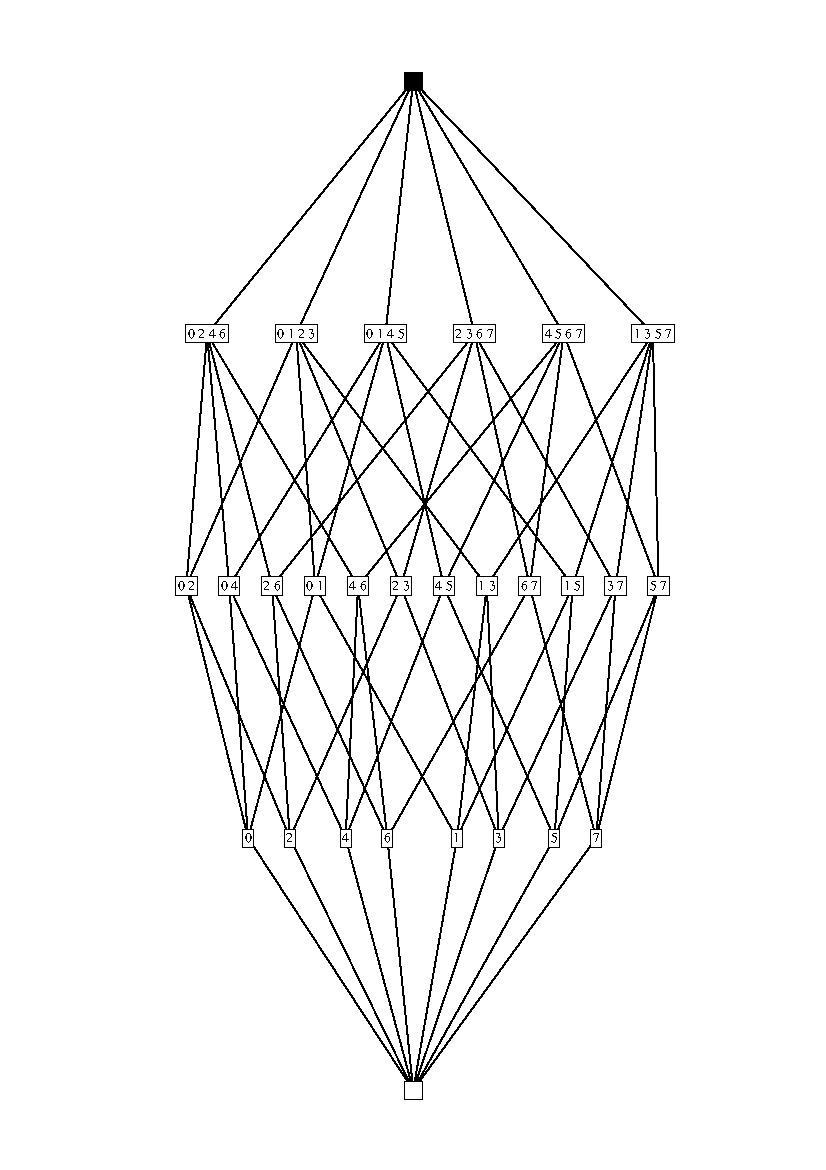
\includegraphics[width=0.9\linewidth]{l6_graph.jpg}
  
  \caption{The representation of the graph of the cube due with Polymake.}
\label{fig:l6:2}
\end{figure}

To see the equations of the facets you can type:

\texttt{polytope > print \$p->FACETS;}

\texttt{1 1 0 0}

\texttt{1 -1 0 0}

\texttt{1 0 1 0}

\texttt{1 0 -1 0}

\texttt{1 0 0 1}

\texttt{1 0 0 -1}

You must interpret as the following:

If you take $(1:1:0:0)$ gives you the facet: 

$$\left\langle(1:1:0:0)\left(\begin{array}{c}
                                                                     1\\	x\\	y\\	z
\end{array}\right)\right\rangle\geqslant 0$$

equivalently: $1+x\geqslant 0$ or $x\geqslant -1$. If you take $(1:-1:0:0)$ gives you the facet: $1-x\geqslant 0$ or $1\geqslant x$.
\newpage
We can polarize a polytope, for example:

\texttt{polytope > \$q=polarize(\$p);}

doing this, if we want to print the vertices of this new polytope, as we expected, gives the facets of the cube:

\texttt{polytope > print \$q->VERTICES;}

\texttt{1 -1 0 0}

\texttt{1 1 0 0}

\texttt{1 0 -1 0}

\texttt{1 0 1 0}

\texttt{1 0 0 -1}

\texttt{1 0 0 1}

Another thing that we can do is make Voronoi Diagrams. For example if we want to know the Voronoi Diagram of the points $(1,1),(0,1),(-1,1),(1,-1),(0,-1)\text{ and }(-1,-1)$:

\texttt{\$VD = new VoronoiDiagram(SITES=>[[1,1,1],[1,0,1],[1,-1,1],}

\texttt{[1,1,-1],[1,0,-1],[1,-1,-1]]);}

If we want to see a graphical representation:

\texttt{\$VD->VISUAL\_VORONOI;}

\begin{figure}[htbp]
  \centering
  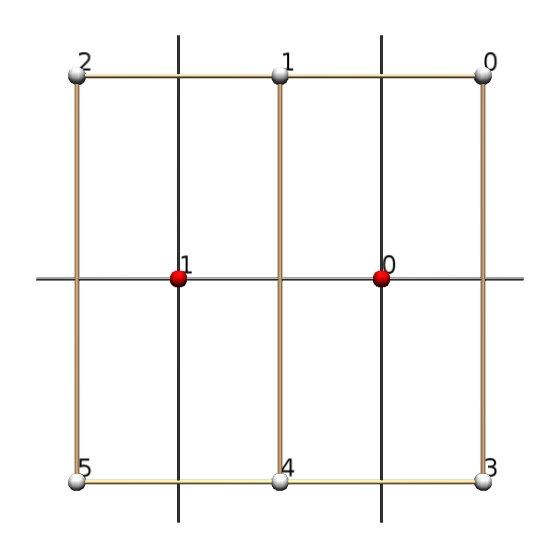
\includegraphics[width=0.7\linewidth]{l6_Voronoi.jpg}
  
  \caption{The representation of one Voronoi Diagram with Polymake.}
\label{fig:l6:3}
\end{figure}
\newpage
Other properties are, for example the facets equation:

\texttt{polytope > print \$VD->FACETS;}

\texttt{2 -2 -2 1}

\texttt{1 0 -2 1}

\texttt{2 2 -2 1}

\texttt{2 -2 2 1}

\texttt{1 0 2 1}

\texttt{2 2 2 1}

\texttt{1 0 0 0}

or the vertices of the diagram:

\texttt{polytope > print \$VD->VERTICES;}

\texttt{0 0 1 2}

\texttt{0 1 0 2}

\texttt{1 1/2 0 -1}

\texttt{0 -1 0 2}

\texttt{0 0 -1 2}

\texttt{1 -1/2 0 -1}

\section{Voronoi Cells in lattices}

Given a lattice $L\subset\RR^d$, find the facets of $$\Vor(0)=\{x\in\RR^d:\|x-0\|^2\leqslant\|x-v\|^2,\forall v\in L\}$$ 

\begin{defn}
 $v\in L$ is \textit{relevant} if the bisector of $v$ and $0$ contains a full dimensional face (i.e. a facet) of $\Vor(0)$.
\end{defn}

In $\ZZ^3$ we have a cube and the polytope defined by the relevant points is an octahedron.

\begin{obs}
 If the relevant vectors are precisely the minimal vector then $\Vor(0)$ is polar dual to the vertex figure of $0$ in $L$.
\end{obs}

\begin{theorem}[Georges Voronoi, 1908]
 A non-zero vector $v\in L$ is relevant if and only if $\pm v$ are the only shortest vectors in the coset $v+2L$.
\end{theorem}

\begin{proof}
 \underline{$\Longrightarrow$}

Suppose that $v,w\in L$ satisfy 

\begin{equation}\label{l6:eq1}
w\in v+2L 
\end{equation}

but

\begin{equation}\label{l6:eq2}
 w\neq \pm v
\end{equation}

and

\begin{equation}\label{l6:eq3}
 \langle w,w\rangle\leqslant \langle v,v\rangle
\end{equation}

Set:

\begin{center}
 $t=\frac{1}{2}(v+w)$ and  $u=\frac{1}{2}(v-w)$
\end{center}

Using (\ref{l6:eq1}) we have that $t,u\neq 0$ and using (\ref{l6:eq2}), $t,u\in L$. We have:

$$H_v=\{x\in\RR^d:\langle x,v\rangle\leqslant \frac{1}{2}\langle v,v\rangle\}$$

Let $x\in H_t\cap H_u$. Then:

$$\langle x,t\rangle\leqslant \frac{1}{2}\langle t,t\rangle$$ 

and

$$\langle x,u\rangle\leqslant \frac{1}{2}\langle u,u\rangle$$

Adding, we have:

$$\begin{array}{rcl}
   \langle x,v\rangle	&\leqslant	&\frac{1}{8}\left(\langle v,v\rangle+\langle w,w\rangle+2\langle v,w\rangle+\langle 							v,v\rangle+\langle w,w\rangle-\langle v,w\rangle\right)\\
			&=		&\frac{1}{4}\left(\langle v,v\rangle+\langle w,w\rangle\right)\\
			&\leqslant	&\frac{1}{2}\langle v,v\rangle
  \end{array}
$$ 

Were in the last one we have used (\ref{l6:eq3}). So $x\in H_v$, therefore $v$ is not relevant.

 \underline{$\Longleftarrow$}
Suppose $v\in L$ is not relevant. Then there exists some $w \in L$. $w\neq 0$, $w\neq \pm v$ with:

\begin{equation}\label{l6:eq4}
 \left\langle \frac{1}{2} v, w\right\rangle \geqslant \frac{1}{2}\langle w,w\rangle
\end{equation}

and $\frac{1}{2}v\notin H_w$.Then

$$\begin{array}{rcl}
   \|v-2w\|^2 	&=		&\langle v-2w,v-2w\rangle \\
		&=		&\langle v,v\rangle - 4 \langle v,w\rangle + 4 \langle w,w\rangle\\
		&\leqslant	&\langle v,v\rangle - 4 \langle v,w\rangle + 4 \langle v,w\rangle\\
		&=		&\langle v,v\rangle
  \end{array}
$$

where in the inequality we have used (\ref{l6:eq4}), and is in $v+2L$, not $0$, $w\in L$.

\end{proof}

% Local Variables: 
% mode: latex
% TeX-master: "dag-upc"
% End: 



\scribe{Ane Santos}



\begin{definition}
Informally, an \emph{orbifold} is the quotient of a manifold (here, the Euclidean plane) by the action of a group.
\end{definition}

\begin{displaymath}
	\begin{array}{lcc}
		torus & \longrightarrow & \circ \\
		holes & \longrightarrow & * \\
		non-orientability & \longrightarrow & \times \\
		boundary singularity & \longrightarrow & *n \\
		core point of order n & \longrightarrow & n \
	\end{array}
\end{displaymath}

\begin{theorem}{Magic theorem for the sphere}
The total cost of the signature of any spherical group is $ \$ 2-frac{2}{g} $ where $g=total number of symmetries$
\end{theorem}

The Magic theorem in the plane is a special case because the number of symmetries in a plane is infinite, so the cost is always 2.

There are 14 spherical symmetry groups: $m,n\geq1$

\begin{displaymath}
	\begin{array}{lcccc}
		*532 & *432 & *332 & *22n & *mn \\
		 & & 3*2 & 2*n & n* \\
		 & & & & n\times \\
		 532 & 432 & 332 & 22n & mn 
	\end{array}
\end{displaymath}

If $n\rightarrow\infty$ and $m\rightarrow\infty$ in $*22n$, $*mn$, $2*n$, $n*$, $n\times$, $22n$ and $mn$ we get the 7 possible groups of friezes (cenefas).

\chapter{Orbifolds}

\scribe{Roger Ten}

\section{Defining an orbifold}

In this section $X$ denotes a topological space and $G$ denotes a topological group. So must begin by defining what is a topological group.

\begin{defn}
\begin{enumerate}
\item A \emph{topological group} is a topological space that is simultaneously a group such that, the group operations are continuous.
\item A topological space $X$ is called \emph{$G$-space} if a topological group $G$ acts on $X$ via a continuous map
 $G\times X \longrightarrow X$, $(g,x)\longmapsto gx$ such that
  $g(hx)=(gh)x$ and $1_Gx=x$.
\end{enumerate}
\end{defn}

\begin{example}
\begin{itemize}
  \item Lie groups: $O(n), SO(n)$
  \item $S^1$ is a topological space and it is also a group via:
  $$\begin{array}[c]{cccc}
 +: &S^1\times S^1&{\rightarrow}&S^1\\
&(\varphi,\psi)&{\rightarrow}& \varphi +\psi
\end{array}$$
\begin{center}
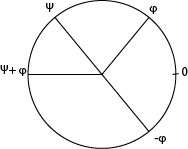
\includegraphics[width=0.5\textwidth]{./suma}
\end{center}
\end{itemize}

\end{example}

Now is coming a list of definitions
\begin{defn}
Let  $x\in X$ be a point.
\begin{enumerate}
\item $G_x=\{g\in G : gx=x\}=Stab_G(x)$ is called the \emph{stabilizer of $x$} or the isotropy subgroup of $x$. $G_x$ is a subgroup of $G$ $(G_x\leqslant G).$
\item $G(x)=\{gx : g\in G\}\subset X$ is the \emph{orbit of $x$}.
\item The action of $G$ on $X$ is \emph{free} if $G_x=\{ 1\} \forall x\in X.$
\item The action of $G$ on $X$ is \emph{transitive} if $G(x)=X \forall x\in X$, i.e., there exist only one orbit.
\item The map $G/G_x\rightarrow G(x)$ is a continuous bijection
\item The orbit space $X/G$ is the set of all orbits in $X$. (It is a topological space with quocient topology).
\item A map $f:X\rightarrow Y$ of $G$-spaces is \emph{$G$-equivariant} (or $G$-map) if $f(gx)=g(f(x)); g\in G$. so the following diagram commutes:
 $$\begin{array}[c]{ccc}
X&\stackrel{f}{\rightarrow}&Y\\
\downarrow\scriptstyle{g}&\circlearrowright&\downarrow\scriptstyle{g}\\
X&\stackrel{f}{\rightarrow}&Y
\end{array}$$
\end{enumerate}
\end{defn}

%---------------------------------------------------- Orbifold Chart

\begin{defn}
An \emph{orbifold chart} on a topological space $X$ is tuple $(\tU,G,\cU, \pi)$, such that:
\begin{itemize}
  \item $\cU\subset X$ is an open subset (neighborhood).
  \item $\tU\subset \RR^n$ is an open subset.
  \item $G$ is a finite group of homomorphisms of  $\tU$.
  \item $\pi:\tU\rightarrow \cU$ can be factorized as $\pi=\tilde{\pi}\circ p$, where 
  $p:\tU\rightarrow \tU/G$ is the orbit map and $\tilde{\pi}:\tU/G\rightarrow \tU$ is an homomorphism.
\end{itemize}
\end{defn}





\begin{tikzpicture}[>=angle 90]
\matrix[matrix of math nodes,row sep=3em, column sep=0.25em,
text height=1.5ex, text depth=0.25ex]
{G&\underset{act\ on}{\circlearrowleft} &|[name=tU]| \tU &\subset &\RR^n \\
     &    &           & &|[name=tUG]| \tU/G \\
& & |[name=U]| \cU & \subset &X \\};
\draw [->,font=\scriptsize]
(tU) edge node[auto] {$p$} (tUG)
(tU) edge node[auto] {$\pi$} (U)
(tUG) edge node[auto] {$\tilde{\pi}$} (U);
\end{tikzpicture}

 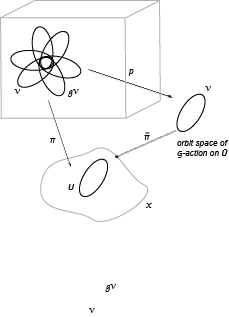
\includegraphics[width=0.5\textwidth]{orbitchart}



 \begin{defn} Two orbifold charts are \emph{compatible} if for all $\tilde{u_i}\in \tU_i,
   i=1,2$ such that $\pi_1(\tilde{u_1})=\pi_2(\tilde{u_2})$ there exists a homomorphism
   $h:\tV_1\rightarrow\tV_2$, where $\tV_i$ is a neighborhood of $\tilde{u_i}$ in $\tU_i$,
   such that $\pi_1=\pi_2\circ h$ on $\tV_1$

\begin{center}
\begin{tikzpicture}[>=angle 90]
\matrix[matrix of math nodes,row sep=1em, column sep=0.5em,
text height=1.5ex, text depth=0.25ex]
{|[name=U2]|\tU_2&\supset &|[name=V2]| \tV_2 & &|[name=V1]|\tV_1&\subset &|[name=U1]| \tU_1 \\
&&&\circlearrowright &&&\\
|[name=U2G]|\tU_2/G& & &|[name=U1U2]| \tU_1\cap\tU_2 & & &|[name=U1G]| \tU_1/G0\\};
\draw [->,font=\scriptsize]
(V1) edge node[auto] {$h$} (V2)
(V1) edge node[auto] {$\pi_1$} (U1U2)
(V2) edge node[auto] {$\pi_2$} (U1U2)
(U1G) edge node[auto] {$\tilde{\pi}_1$} (U1U2)
(U2G) edge node[auto] {$\tilde{\pi}_2$} (U1U2)
(U1) edge node[auto] {$p_1$} (U1G)
(U2) edge node[auto] {$p_2$} (U2G);
\end{tikzpicture}
\end{center}
\end{defn}

\begin{remark}
$G_i=\{1\}$ yields manifolds.
\end{remark}

\begin{defn}
An \emph{orbifold atlas} is a collection of compatible orbifold charts that cover $X$.\\
An \emph{orbifold $Q$} is an underlying Hausdorff topological space $|Q|$ with an orbifold atlas.
\end{defn}

\section{Covering orbifolds}

A \emph{covering} of a topological space $X$ is a topological space $Y$, together with a
continuous surjective projection $\pi: Y\rightarrow X$ such that for every $x\in X$ exist
$\cU_x$ open neighborhood of $x$ such that the pre-image $\pi^{-1}(\cU_x)$ is a disjoint
union of copies of $\cU_x$.


\begin{defn}
A \emph{covering orbifold} of an orbifold $Q$ is an orbifold $\tilde{Q}$ with a projection $\pi:|\tilde{Q}|\rightarrow|Q|$ between the underlying spaces with the following property:
\begin{quote}
  For any $x\in |Q|$ there exist a neighborhood $\cU\cong \tU/G$; $\cU\subset \RR^n$ such
  that each connected component $C$ of $\pi^{-1}(\cU)$ is homeomorphism to $\tU/\Gamma_i$
  for some subgroup $\Gamma_i\leqslant G$.
\end{quote}
\end{defn}
\begin{remark}
This homeomorphism $\varphi$ must respect both projections, namely $\pi$ and $p_i:\tU/G\rightarrow\tU/\Gamma_i$.

\vspace*{2cm}
\begin{tikzpicture}[>=angle 90]
\matrix[matrix of math nodes,row sep=1em, column sep=3em,
text height=1.5ex, text depth=0.25ex]
{&&&&\\
|[name=tQ]| |\tilde{Q}|&|[name=C]| 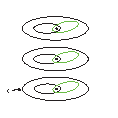
\includegraphics[width=0.15\textwidth]{./C} & &|[name=tU]|\tU &|[name=tUd]| 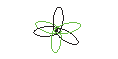
\includegraphics[width=0.15\textwidth]{./tU} \\
&&&&\\
 &&\circlearrowright & |[name=tUG]| \tU/G& |[name=tUGd]| \\
|[name=Q]| |Q|&|[name=U]|  \cU & & &
\includegraphics[width=0.15\textwidth]{./tUG} \\
&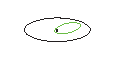
\includegraphics[width=0.15\textwidth]{./U}&&&\\};
\draw [->,font=\scriptsize]
(tQ) edge node[auto] {$\pi$} (Q)
(C) edge node[auto] {$\pi$} (U)
(tUG) edge node[auto] {$\tilde{\pi}$} (U)
(tU) edge node[auto] {$\varphi$} (C)
(tU) edge node[auto] {$p$} (tUG)
(tUd) edge node[auto] {$p$} (tUGd);
\end{tikzpicture}


\end{remark}

\begin{defn}
An orbifold is called \emph{good} or developable if there exists some manifold that covers it. Otherwise, it is \emph{bad} or not developable
\end{defn}



% Local Variables: 
% mode: latex
% TeX-master: "dag-upc"
% End: 

\chapter{The Magic Theorem}

\scribe{Victor Bravo}

Today, we want to prove the Magic Theorem. To do this, we will introduce the language of the CW-Complexes: \newline

\underline{CW-COMPLEXES:}
\begin{obs} The theory of CW-Complexes was developed around 1910 by J.H.\underline{C}. \underline{W}hitehead. Also, the 'C' do refence to 'closed' and the 'W' do reference to 'weak' in the sentence 'closed in the weak topology'. \newline
We will use CW-Complexes to generalize triangulations of the space.
\end{obs}

Let $X$ be a topological space. \newline
We define $X^{0} := 0$-skeleton of $X = \lbrace \text{points in } X \rbrace$. \newline
Inductively, given the $(n-1)$-skeleton of $X$, take a bunch of $n$-dimensional closed disks ($\equiv$ balls) $e_{1}^{n}, \ldots, e_{r}^{n}$, and we can do the next attaching map $\varphi _{i} : \mathbb{S}^{n - 1} = \partial e_{i}^{n} \longrightarrow X^{n - 1}$. \newline
$X^{n} := X^{n-1} \stackrel{\bullet}{\bigcup}_{i} e_{i}^{n} / \sim$, where $x \sim \varphi_{i}(x)$. \newline
Since a $1$-dimensional disk is an interval, taking a set of points in a plane, a $1$-dimensional CW-Complex is a multigraph with loops. \newline
In dimension $2$, a good example can be to take only the point $p$ as the $0$-skeleton, an empty number of $1$-dimensional balls, and a $2$-dimensional ball (which is a disk). So, we have that the attaching map goes from the boundary of this disk (which is $\partial e^{2} = \mathbb{S}^{1}$) to the lower dimensional skeleton (which is the point $p$). Doing the $\sim$, we get the $2$-dimensional sphere. \newline
The same example works for any dimension $n$ using stereographic projection. So, we can calculate the number of cells that we need to decomposing $\mathbb{S}^{n}$ as a regular triangulation (regular in the sense of not having identifications on the boundary of the cell and in the sense of the intersection of two faces is empty or a face of both). \newline
For dimension $0$, we have two points. So, the $f$-vector of $\mathbb{S}^{0}$ is $(2)$ (which means: two $0$-dimensional faces), and we need $(2)$ cells in the CW-complex. \newline
For dimension $1$, we have $\mathbb{S}^{1}$ and, to do a regular triangulation, we need three different distinguished points. So, the $f$-vector of $\mathbb{S}^{1}$ is $(3, 3)$ (which means: three $0$-dimensional faces and three $1$-dimensional faces), and we need $(1, 1)$ cells in the CW-complex. \newline
For dimension $2$, we have $\mathbb{S}^{2}$ and, to do a regular triangulation, we need a tetrahedron over the $\mathbb{S}^{2}$ surface. So, the $f$-vector of $\mathbb{S}^{2}$ is formed by $4$ vertices, $\binom{4}{2}$ edges, and $\binom{4}{3}$ faces (triangles). This is $(4, 6, 4)$, and we need $(1, 0, 1)$ cells in the CW-complex. \newline
For dimension $n$, we have the $n$-dimensional simplex. So, whose $f$-vector is equal to $(n + 1, \binom{n+1}{2}, \binom{n+1}{3}, \ldots, \binom{n+1}{n})$ (that has $2^{n+1}-2$ elements), and we need $(1, 0, \ldots, 0, 1)$ cells in the CW-complex. \newline

To go towards the Magic Theorem, we need to remember the definition of the covering of an orbifold to explain: \newline

\underline{THE ORBIFOLD EULER CHARACTERISTIC:} \newline \newline
Let be $G$ a group that acts over an orbifold $Q$, $G \circlearrowleft Q$. \newline
So, taking $x \in Q$, we have that $G_{x} \leq G$ is that we call the stabilizer of $x$. \newline
What we want to do is to decompose $Q$ as a CW-complex into invariant cells, i.e., into a collection, $\mathcal{C}$, of cells such that the function $x \mapsto G_{x}$ is constant on each cell, $C \in \mathcal{C}$ (observe that $C^{0} \subset C$). \newline
An example of this is to take $\vert Q \vert = \mathbb{D}^{2}$ and $G$ as the abstract group $G = \lbrace e = id, g, g^{2} \rbrace = \mathbb{Z}_{3}$, where $g$ represents a rotation of $\frac{2 \pi}{3}$ (this is the same that to think in $G$ as the spherical group formed by two rotation points of order three). Now, we want to decompose this as a CW-manifold into cells such that the stabilizing subgroup is constant. We have two differents types of points that we resume as points $y$, which are rotation points, and points $x$ which are not rotation points. Now, the stabilizing group of the points $x$ is $G_{x} = \lbrace e \rbrace$, and the stabilizing group of the points $y$ is $G_{y} = G$. So now, we will have to decompose this disk as a CW-complex made-up of invariant cells. To do this, we have to leave one of the rotation points in the interior of the disk, the other rotation point over the boundary of the disk, and add two new points over the boundary of the disk. \newline
Now, we define the \textsl{Euler Characteristic of an orbifold} as $$\chi (Q) = \sum_{C \in \mathcal{C}} \frac{(-1) \dim C}{\# G_{C}}.$$
To see that this definition works, we have to check two things. \newline
The first thing is that this defition is an application of the original Euler Characte-ristic that works over orbifolds in the same sense of the original works over simplicial complexes, where the original Euler Characteristic is defined as the alternating sum of the $f$-vector of the simplicial complex.
\begin{example} Taking the simplicial complex formed by the three vertices, the three edges and the face of a triangle (i.e., a $2$-dimensional ball), we have to sum $1(-1)^{2}$ for the face, $3(-1)^{1}$ for the edges, $3(-1)^{0}$ for the vertices and $1(-1)^{-1}$ for the $\emptyset$, which gives us $\chi = 0$. \newline
In the same way, if we take the simplicial complex formed by the three vertices, the three edges of a triangle, this gives us $\chi = -1$. \newline
\end{example}

This works for any regular triangulation, so, if works for orbifolds. \newline
The second thing to check is that this formula works for the group, but in the case of having a simplicial complex there is no group, or in other words, we have only the identity. So, it works for the group. \newline
Now, what we really wants is apply this to coverings, so, remember: \newline
In a $k$-fold, covering $\tilde{Q} \rightarrow Q$ of orbifolds, every point in $\vert Q \vert$ has $k$ pre-images. \newline
\begin{theorem} If $\tilde{Q} \rightarrow Q$ is a $k$-fold covering of orbifolds, then $\chi(\tilde{Q}) = k \chi (Q)$.
\end{theorem}
\begin{proof} Remembering session 9, let $y \in U$ be a non-singular point in an orbifold chart, $U$, which corresponds to a some number of points in $V$. \newline
The number of pre-images of $y$ in each neighborhood of $\tilde{x}_{i}$ is $\dfrac{\vert G_{x} \vert}{\vert G_{\tilde{x}} \vert}$. \newline
So, the total number of preimages of $y$ is $$k = \sum_{\tilde{x} \in \Pi ^{-1}(x)} \frac{\vert G_{x} \vert}{\vert G_{\tilde{x}} \vert},$$ which implies that $$\frac{k}{\vert G_{x} \vert} = \sum _{\tilde{x} \in \Pi ^{-1}(x)} \frac{1}{\vert G_{\tilde{x}} \vert}.$$ Now, using that the cells are invariant and $x \mapsto G_{x}$, we have that $$\frac{k}{G_{x}} = \frac{k}{G_{C}}.$$ So, we have that $$k \chi (Q) = \sum_{C \in \mathcal{C}} \frac{k (-1)^{\dim (C)}}{\vert G_{C} \vert} = \sum _{\tilde{C} \in Pi^{-1}(C)} \frac{(-1)^{\dim (C)}}{\vert G_{\tilde{C}} \vert} = \chi (\tilde{Q}),$$ where the last equality holds because $\tilde{C} \in Pi^{-1}(C), \forall C \in \mathcal{C}$, and this sums over all $\tilde{C} \in \vert \tilde{Q} \vert$.
\end{proof}
\qed

\begin{example} Let's take $\vert Q \vert = \mathbb{D}^{2}$ with $k$ mirrors and $k$ corner reflectors  labeled $m_{1}, \ldots, m_{k}$. \newline
If we compute de signature of this, we have no blue part because there are not rotation points. Then, we have a \textcolor{red}{$*$}, and we can take, for example, the signature \textcolor{red}{$*632$}. So, we have one point, $A$, with $6$ mirrors through it, another point, $C$, with $3$ mirrors through it, and another point, $B$, with $2$ mirrors through it. Now, if we go down to the orbifold (taking one copy of every mirror), we have $3$ mirrors in the orbifold. So, $k = 3$. Now, we want to cellulate this CW-complex such that every cell in the CW-complex has the same stabilizer. Since, $A$ is stabilized by the subgroup $D_{6}$, $B$ is stabilized by the subgroup $D_{2}$, and $C$ is stabilized by the subgroup $D_{3}$, we can compute the Orbifold Euler Characteristic. \newline
We have, for dimension $0$, $$\frac{(-1)^{0}}{\vert D_{6} \vert} + \frac{(-1)^{0}}{\vert D_{2} \vert} + \frac{(-1)^{0}}{\vert D_{3} \vert},$$ for dimension $1$, $$\frac{(-1)^{1}}{\vert \mathbb{Z}_{2} \vert} + \frac{(-1)^{1}}{\vert \mathbb{Z}_{2} \vert} + \frac{(-1)^{1}}{\vert \mathbb{Z}_{2} \vert},$$ and for dimension $2$, $$\frac{(-1)^{2}}{\vert \lbrace e \rbrace \vert}.$$ \newline
So, $$\tilde{\chi} = \frac{1}{12} + \frac{1}{4} + \frac{1}{6} - \frac{1}{2} - \frac{1}{2} - \frac{1}{2} + \frac{1}{1} = 0.$$
\end{example}

\begin{example} Doing the same example with any $k$ corner reflectors using the notation $m_{i}$ to note the number of mirrors through the corner $i$, we will have $$\tilde{\chi} = \sum_{i = 1}^{k} \frac{1}{2 m_{i}} - \frac{k}{2} + 1 = \frac{1}{2} \sum_{i = 1}^{k} \left(\frac{1}{m_{i}}\right) + 1 = 1 - \sum_{i=1}^{k} \frac{m_{i} - 1}{2 m_{i}}.$$ So, if we get a disk, it has this Euler Characteristic.
\end{example}

\begin{example} Now, an example with true-blue signature (which means that we have only rotation points). Let's take $\vert Q \vert = \mathbb{S}^{2}$, and $l$ cone points labeled $n_{1}, \ldots, n_{l}$. Let's take, for example, \textcolor{blue}{$532$} over $\mathbb{S}^{2}$. So, we have a sphere and three cone points. The first thing we've got to do is to cellulate the sphere as a CW-complex such that each cell has constant stabilizer. So, it seems very clear that we are going to use $0$-dimensional vertices at the cone points. So, the stabilizing subgroup is $C_{5}$ for one point, $C_{3}$ for another point, and $C_{2}$ for another point. In the same way, the stabilizing subgroup of the edges that goes from one point to another is $\lbrace e \rbrace$, and also for the face, the subgroup is $\lbrace e \rbrace$. So, we have that $$\tilde{\chi} = \frac{(-1)^{0}}{5} + \frac{(-1)^{0}}{3} + \frac{(-1)^{0}}{2} - 1 - 1 - 1 + 1 + 1 = \sum_{i = 1}^{l} \frac{1}{n_{i}} - l + 2 = 2 - \sum_{i = 1}^{l} \frac{n_{i} - 1}{n_{i}}.$$
What we have to observe here is that seems that we extract something from $2$. In the last example seems that happens the same thing, but there we had a \textcolor{red}{$*$} and all was natural. What happens here is that using $\chi({\mathbb{S}^{2}}) = (-1)^{0} + (-1)^{2} = 2$, we have that if we do a hole over the sphere, we are substracting $1$, because $\chi(\mathbb{S}^{2} \text{ with a hole}) = 1$, and we have the possible \textcolor{red}{$*$}'s covered. So, finally we have that $\tilde{\chi}(Q) = 2 - (\text{cost of the signature})$.
\end{example}



% Local Variables: 
% mode: latex
% TeX-master: "dag-upc"
% End: 

\chapter{Quasicrystals}
\begin{figure}[h] %[h] para here [b] para bottom [t] para top
\centering
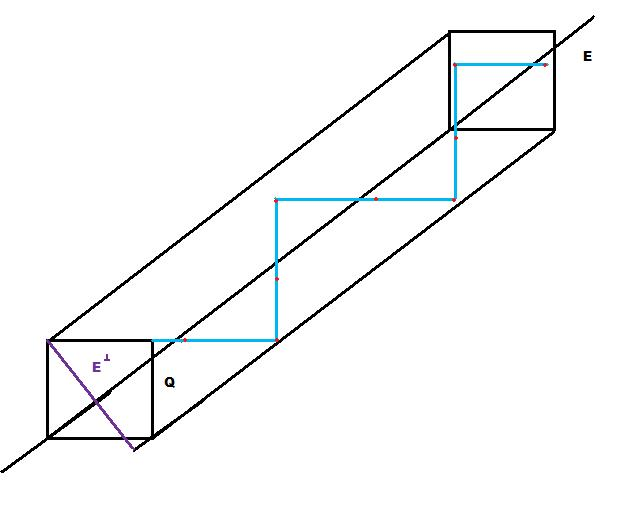
\includegraphics[width=250pt]{./graphics/Quasi.jpg}
%\caption{Ejemplos de cada tipo de juego}
\end{figure}
We pick
$$\textbf{E}=\{\vec{x}\in\RR^2\ |\ x_2=x_1\cdot c,\ c\in\RR\setminus\QQ\}.$$
There are $2$ kind of segments the big ones and the smaller ones the proportion is $c$.\smallskip\\
$\textbf{E}^{\bot}$ is dense $\Rightarrow 2^{\NN}$ is $\infty$ no countable.\smallskip\\
We can generalize this to any parallelepiped and if we are in a lattice the canonical projetion method picks $\Vor(0)$ as $Q$. It is also possible in higher dimensions.\smallskip\\
Given $x\in L$, $\textbf{E}\subset \RR^d$, $Q\subseteq\RR^d$ we have to decide whether $x\in\mathbf{E}+Q$.\smallskip\\
We project $Q$ and $x$ onto $\pi_{\textbf{E}^{\bot}}(\mathbf{E}+Q)$, where $\pi_{\textbf{E}^{\bot}}$ is the projection window, if $x^{'}\in Q^{'}\Leftrightarrow x\in\mathbf{E}+Q$.

\bibliographystyle{amsalpha}
\bibliography{dag}

\end{document}

%%% Local Variables: 
%%% mode: latex
%%% TeX-master: t
%%% End: 
